\documentclass[classical]{einfart}
\usepackage{ProjLib}
\usepackage{hologo}
\usepackage{graphicx} %插入图片的宏包
\usepackage{float} %设置图片浮动位置的宏包
\usepackage{subfigure} %插入多图时用子图显示的宏包
\usepackage{hyperref}
% \usepackage{ctex} % 中文的宏包

\setCJKmainfont{Noto Serif CJK TC} % 主要字體 Noto Serif
% \UseLanguage{TC}
%%================================
%% Titles
%%================================
\let\LevelOneTitle\section
\let\LevelTwoTitle\subsection
\let\LevelThreeTitle\subsubsection

\providecommand{\tightlist}{%
  \setlength{\itemsep}{0pt}\setlength{\parskip}{0pt}}

\begin{document}

% \setcounter{tocdepth}{2}
% {\setstretch{1.07}\tableofcontents}

% \newpage

\part{個人能力}

\section{技術背景}

\begin{itemize}[parsep=0.5ex]
    \item \textbf{程式語言}: $C++, C, JavaScript, Java, Python$.
    \item \textbf{平臺}: Windows, ArchLinux.
    \item \textbf{開發}: 熟練使用 VueJS 前端框架、Flask 微服務框架、MySQL 資料庫。
    \item \textbf{主修專業課程}: 計算機程式設計基礎(C++)、數據結構、Web應用開發技術、演算法分析與設計、計算機網路原理、軟體開發架構平台、資料庫系統SSD7、軟體體系結構、機器學習與資料探勘。
    \item \textbf{Github}:\href{https://github.com/HuangNO1}{https://github.com/HuangNO1}
    \item \textbf{個人Blog}:\href{huangno1.github.io}{huangno1.github.io}
\end{itemize}

\begin{figure}[H]
  \centering
  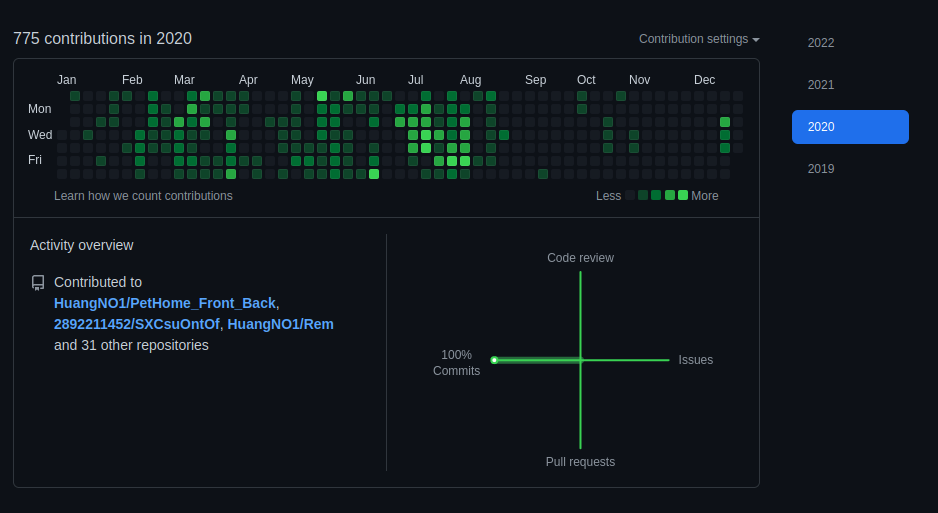
\includegraphics[width=1\textwidth]{img/2020_github.png}
  \caption{GitHub}
\end{figure}

\newpage

\part{專案}

本人的開發經驗包含:

\begin{itemize}[parsep=0.5ex]
  \item \textbf{WEB應用開發(全端)}
  \item \textbf{桌面應用開發(Qt)}
  \item \textbf{Android應用開發(Java)}
  \item \textbf{嵌入式應用開發(Modbus)}
\end{itemize}

\section{校內合作專案}

\textbf{仿 QQ 通訊軟體 (Qt C++、Golang、Gorilla WebSocket、SQLite)} \hfill 2019-07 $\sim$ 2019-08

\begin{itemize}[parsep=0.5ex]

  \item \textbf{項目Github}:
  
  \begin{itemize}[parsep=0.5ex]
    \item Qt 前端:\href{https://github.com/junyussh/MumiChat-Client}{https://github.com/junyussh/MumiChat-Client}
    \item Golang 後端:\href{https://github.com/junyussh/MumiChat-server}{https://github.com/junyussh/MumiChat-server}
  \end{itemize}

  \item \textbf{成效與結果}:此項目實現桌面端通訊軟體,可以基本的使用者登入註冊、好友管理、與多個好友在線聊天發送訊息。

\end{itemize}

\newline

\textbf{基於 JSP 技術實現寵物商店網站 (JSP、Tomcat、MySQL、JQuery)} \hfill 2019-09 $\sim$ 2019-12

\begin{itemize}[parsep=0.5ex]

  \item \textbf{成效與結果}:基本的使用者登入註冊、商品購買添加購物車、結帳、網頁CSS主題切換。後端有配置日誌查看行為。

\end{itemize}

\newline

\textbf{動畫網站 (VueJS、Django)} \hfill 2019-10 $\sim$ 2019-12

\begin{itemize}[parsep=0.5ex]

  \item \textbf{項目Github}:
  
  \begin{itemize}[parsep=0.5ex]
    \item VueJS 前端:\href{https://github.com/HuangNO1/anime_web_vue}{https://github.com/HuangNO1/anime\_web\_vue}
    \item Django 後端:\href{https://github.com/2892211452/JK-DM}{https://github.com/2892211452/JK-DM}
  \end{itemize}

  \item \textbf{成效與結果}:固定時間爬取其他網頁的API將其視頻資源來源寫入本地資料庫,網頁能夠做到搜索播放、發送彈幕、主要針對使用者體驗去做UI設計,包括紀錄使用者播放紀錄。

\end{itemize}

\newline

\textbf{基於微空運輸的移植器官運輸路徑規劃系統 (VueJS、Flask)} \hfill 2020-01 $\sim$ 2020-10

\begin{itemize}[parsep=0.5ex]

  \item \textbf{成效與結果}:在一次搜索中能在10秒內完成複雜的路徑演算法推算,並給出三個路線規劃分別為空中直飛、城市多點陸運與空運交替(看交通是否壅塞)、多個空運中轉點。

\end{itemize}

\newline

\textbf{基於前後端完全分離實現寵物商店 (VueJS、SpringBoot、MySQL)} \hfill 2020-03 $\sim$ 2020-06

\begin{itemize}[parsep=0.5ex]

  \item \textbf{項目Github}:
  
  \begin{itemize}[parsep=0.5ex]
    \item VueJS 前端:\href{https://github.com/HuangNO1/PetHome_Front_Back}{https://github.com/HuangNO1/PetHome\_Front\_Back}
    \item SpringBoot 後端:\href{https://github.com/lumusen0305/springBoot-vue}{https://github.com/lumusen0305/springBoot-vue}
  \end{itemize}

  \item \textbf{成效與結果}:在之前的寵物商店專案上更進一步完成網頁開發後端完全分離架構,除了完成前臺購物,進一步完成後臺管理員頁面管理,對於商品的TAG更有效率搜索種類。

\end{itemize}

\newline

\textbf{個人空間系統 (VueJS、SpringBoot、Flask、MySQL)} \hfill 2020-07 $\sim$ 2020-08

% 項目角色: \quad 技術開發人員
\begin{itemize}[parsep=0.5ex]
\item \textbf{項目Github}: \href{https://github.com/2892211452/SXCsuOntOf}{https://github.com/2892211452/SXCsuOntOf}

\item \textbf{成效與結果}:部落格系統對應學校學生使用,使用 Vue 實現關於部落格平台的Markdown文章編輯、發表、收藏、用戶資訊修改等
,並使用爬蟲爬取新聞資訊整合成功能模組介面,MySQL儲存用戶訊息、文章訊息、文章Tag等。

\end{itemize}

\newline

\textbf{簡易版今日頭條 (Android Java)} \hfill 2021-05 $\sim$ 2021-06

% 項目角色: \quad 個人開發

\begin{itemize}[parsep=0.5ex]
\item \textbf{項目Github}: \href{https://github.com/HuangNO1/TouTiao_Simple_Android_App}{https://github.com/HuangNO1/TouTiao\_Simple\_Android\_App}

\item \textbf{主要職責與業績}:安卓應用開發課程項目與字節跳動(ByteDance)用戶端合作,技術層面針對重複需要渲染的文字卡片等進行抽象組件化
,避免一次請求渲染太多資料,所以設計結構上,一次請求固定資料,不夠再緩加載更多請求。圖片也做緩存動作,有效解決圖片加載緩慢問題。

\end{itemize}

\section{實習專案}

\textbf{智慧網關應用開發 (Nanopi、C、Modbus、FTP、Vue、Flask)} \hfill 2021-11 $\sim$ 2022-02

% 項目角色: \quad 項目開發人員
\begin{itemize}[parsep=0.5ex]
\item \textbf{成效與結果}:使用 Modbus 協議讀取多個物聯網裝置的信號變化至共享記憶體,
針對信號變化異常用 FTP 傳輸裝置的異常日誌,一個物聯網網關能多線程20個物聯網裝置,響應速度0.01秒,
網頁能夠相當於一個嵌入式系統控制網關的運行參數,像是IP、資料庫、開關機、Modbus協議設定等。

\end{itemize}

\section{畢業後外包專案}

\textbf{施工現場盤點緩存APP (AngularJS、Ionic、Android、IOS)} \hfill 2022-08 $\sim$ 2022-09

\begin{itemize}[parsep=0.5ex]
\item \textbf{成效與結果}:使用Angualr2利用Ionic套件開發非原生應用,達到跨平台使用,此應用能連線伺服器下載現場施工表單,並在離線狀態下簽名、拍照、盤點現場器具狀態,最後在有網路的狀況下連線伺服器上傳資料。

\end{itemize}

\newpage

\part{榮譽與獎學金}

\section{高中}

\subsection{2016}

\begin{itemize}[parsep=0.5ex]
  \item \textbf{文藝與編輯營寒訓}
\end{itemize}

\subsection{2017}

\begin{itemize}[parsep=0.5ex]
  \item \textbf{臺灣師範大學大學先修課程}

  \item \textbf{APCS七級分}
  
  \item \textbf{校內資訊程式競賽佳作}
\end{itemize}

\section{大學}

備註:大學生創新創業項目是全國性性質,單個學校申請件數包含本科生研究生共數千件,本校每年僅200餘件能評定省級或國家級。

\subsection{2019}

\begin{itemize}[parsep=0.5ex]
  \item \textbf{QST 青軟實訓}

  \item \textbf{2019 年度台灣、港澳及華僑學生獎學金 \quad 三等獎}
\end{itemize}

\subsection{2020}

\begin{itemize}[parsep=0.5ex]
  \item \textbf{大學生創新創業項目校級評定}

  \item \textbf{交通科技運輸大賽 \quad 校級一等獎}
\end{itemize}

\subsection{2021}

\begin{itemize}[parsep=0.5ex]
  \item \textbf{全國大學生電子商務“創新、創意及創業”挑戰賽 \quad 校級二等獎}

  \item \textbf{大學生創新創業項目省級評定}
  
  \item \textbf{2021 年度台灣、港澳及華僑學生獎學金 \quad 二等獎}
\end{itemize}

\subsection{2022}

\begin{itemize}[parsep=0.5ex]
  \item \textbf{大學生創新創業項目省級評定}

  \item \textbf{優等畢業論文--“基於狀態檢測的網關優化與可視化”}
\end{itemize}

\newpage

\section{校外實習}

\textbf{上海鈞盟實業有限公司 \quad 研發工程師} \hfill 2021-09 $\sim$ 2022-04

\textbf{主要職責與業績}: \quad 負責大全賽雪龍、ORing、Moxa等客戶的智慧網關應用開發,
使用工業物聯網的相關協議結合網頁開發技術解決裝置的狀態的讀取、
網關系統可視化操作等,將公司舊的Web1.0(基於PHP語言編寫、
GET POST混用)網關控制頁面功能重構設計升級Web2.0
(基於Vue2.0與Flask,重整後端介面為 Restful API風格),提高用戶的使用體驗與功能。

\begin{figure}[H]
  \centering
    \subfigure[實習鑑定表]{\label{Fig.sub.1}
    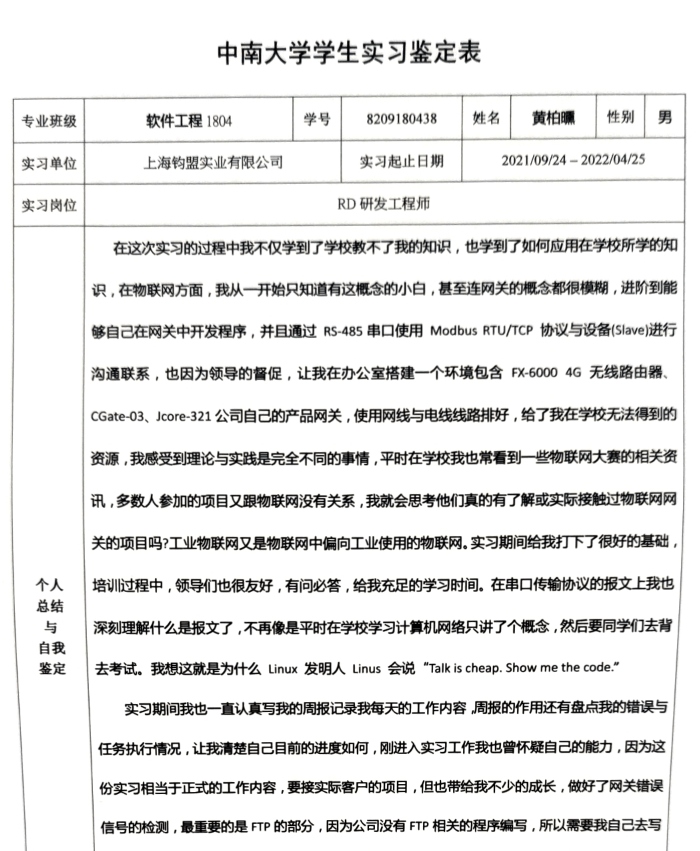
\includegraphics[width=0.4\textwidth]{img/fieldwork_1-min.png}}
    \subfigure[蓋章證明]{\label{Fig.sub.1}
    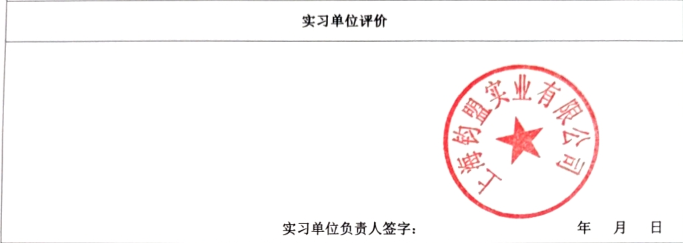
\includegraphics[width=0.4\textwidth]{img/fieldwork_3.png}}
    \caption{中南大學外出實習鑑定}
\end{figure}

\section{大學前簽約Offer}

\begin{figure}[H]
  \centering
  \includegraphics[width=0.5\textwidth, angle=180]{img/offer-min.jpg}
  \caption{大四期間獲得大公司Offer}
\end{figure}

% ---------------------------------------------------
\newpage

\part{附錄}

\begin{figure}[H]
  \centering
  \includegraphics[width=0.5\textwidth, angle=90]{img/2016_school_literature-min.jpg}
  \caption{文藝與編輯營寒訓證書}
\end{figure}

\begin{figure}[H]
  \centering
  \includegraphics[width=0.7\textwidth, angle=180]{img/2017_school_ntnu_C-min.jpg}
  \caption{臺灣師範大學大學先修課程證書}
\end{figure}

\begin{figure}[H]
  \centering
  \includegraphics[width=0.7\textwidth, angle=90]{img/2017_apcs-min.jpg}
  \caption{APCS 考試成績單}
\end{figure}

\begin{figure}[H]
  \centering
  \includegraphics[width=0.5\textwidth]{img/2017_school-min.jpg}
  \caption{中正高中校內資訊競賽佳作獎狀}
\end{figure}

\begin{figure}[H]
  \centering
  \includegraphics[width=0.5\textwidth, angle=90]{img/2019_qst-min.jpg}
  \caption{QST 青軟實訓證書}
\end{figure}

\begin{figure}[H]
  \centering
    \subfigure[結題獎狀]{\label{Fig.sub.1}
    \includegraphics[width=0.3\textwidth, angle=90]{img/2020_-min.jpg}}
    \subfigure[榮譽獎狀]{\label{Fig.sub.1}
    \includegraphics[width=0.3\textwidth, angle=90]{img/2020_1-min.jpg}}
    \caption{大學生創新創業項目獎狀}
\end{figure}

\begin{figure}[H]
  \centering
  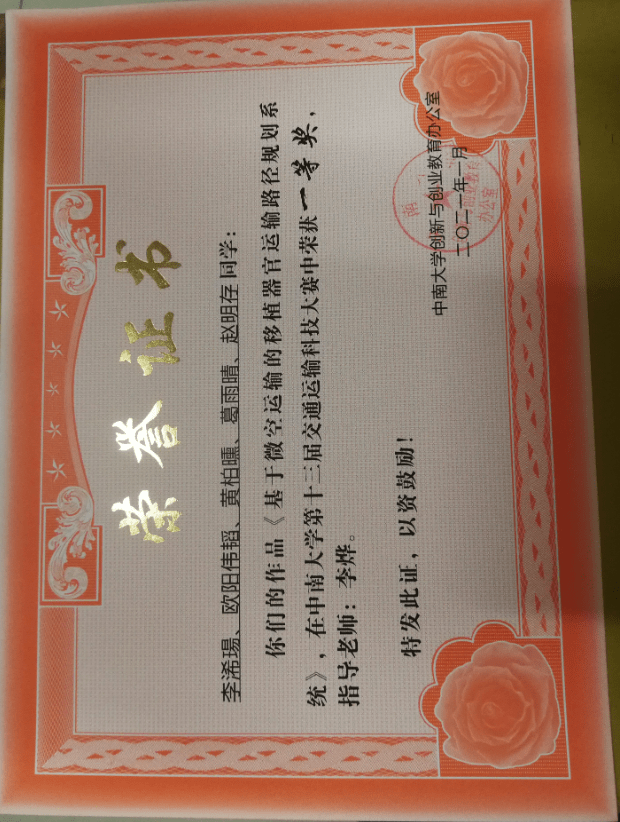
\includegraphics[width=0.5\textwidth, angle=270]{img/2021_traffic-min.png}
  \caption{交通科技運輸大賽獎狀}
\end{figure}

\begin{figure}[H]
  \centering
  
\includegraphics[width=0.5\textwidth]{img/三創賽獎狀-min.jpg}
  \caption{三創賽獎狀}
\end{figure}

\begin{figure}[H]
  \centering
  
\includegraphics[width=0.5\textwidth]{img/2021_-min.png}
  \caption{大學生創新創業結題證明}
\end{figure}

\end{document}